\chapter{System requirement and specification}


\section{Use Case diagrams}
\subsection{Use Case - System Component}

%add your use case diagrams here

\begin{figure}[H]
\centering
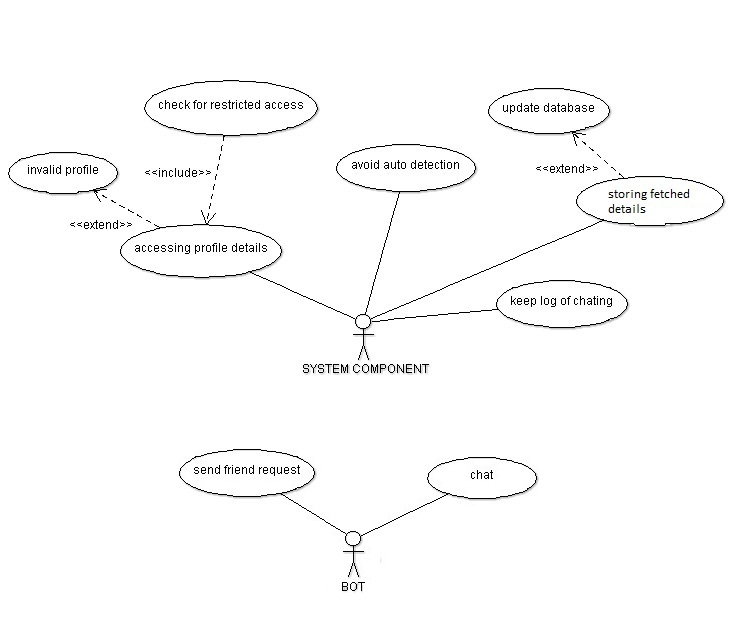
\includegraphics[scale=0.7]{project/diagrams/usecase1}
\caption{Use Case Diagram - System Component}
\label{fig:usecase1}
\end{figure}

\begin{figure}[H]
\centering
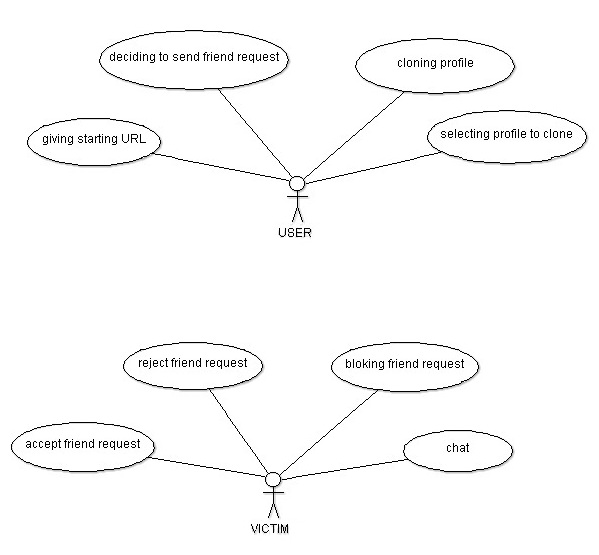
\includegraphics[scale=0.8]{project/diagrams/usecase2}
\caption{Use Case Diagram - Victim and User}
\label{fig:usecase2}
\end{figure}

\begin{figure}[H]
\centering
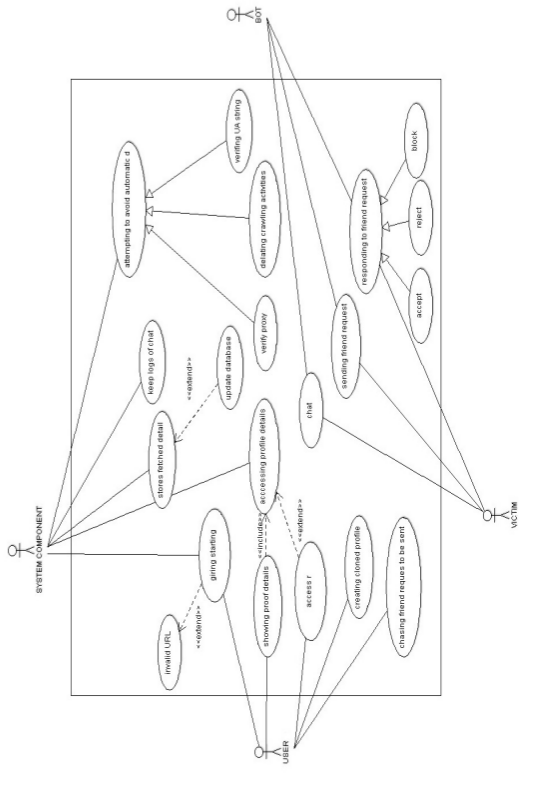
\includegraphics[scale=1.0]{project/diagrams/usecase3}
\caption{Use Case Diagram - Main}
\label{fig:usecase3}
\end{figure}


%Add more if you have to with copy pasting subsections


%add your ER diagrams here
\section{ER Diagram}


\begin{figure}[H]
\centering
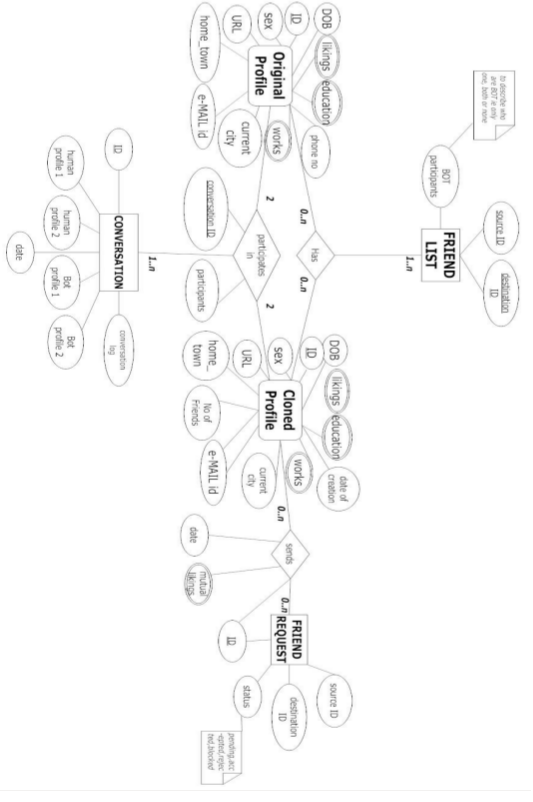
\includegraphics[scale=1.0, angle=180]{project/diagrams/er1}
\caption{ER Diagram}
\label{fig:er}
\end{figure}



\section{DFD (level 0/1/2)}

\subsection{DFD Level 0}

\begin{figure}[H]
\centering
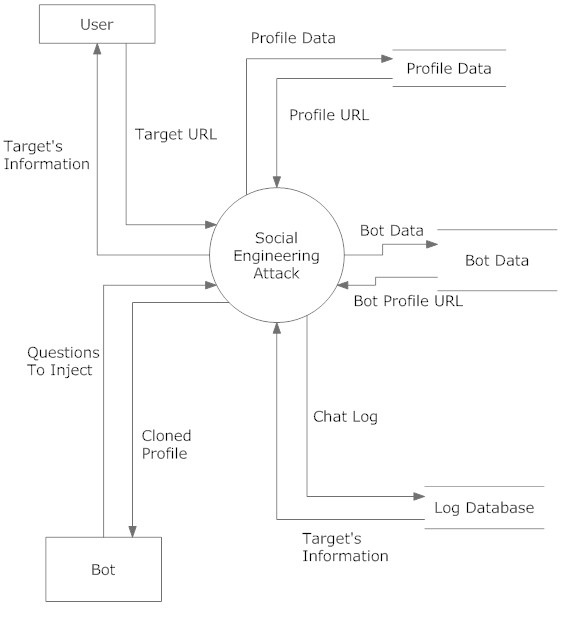
\includegraphics[scale=0.8]{project/diagrams/dfd0}
\caption{DFD - Level 0}
\label{fig:dfd0}
\end{figure}

\subsection{DFD Level 1}

\begin{figure}[H]
\centering
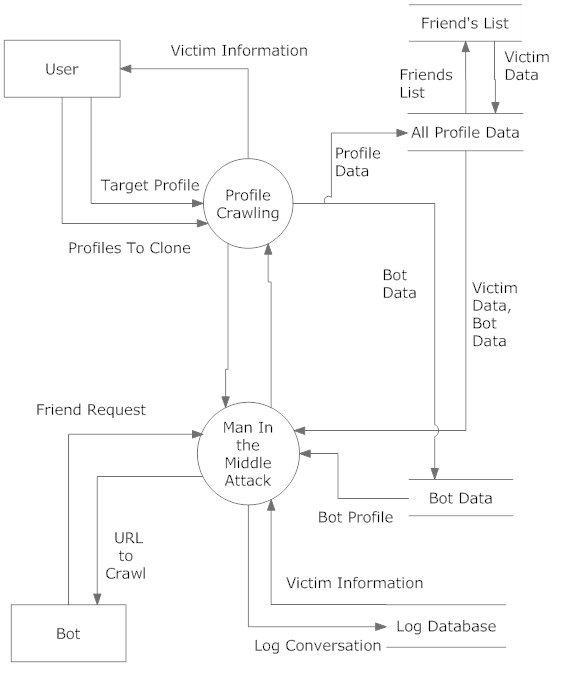
\includegraphics[scale=0.8]{project/diagrams/dfd1}
\caption{DFD - Level 1}
\label{fig:dfd1}
\end{figure}

\subsection{DFD Level 2}

\begin{figure}[H]
\centering
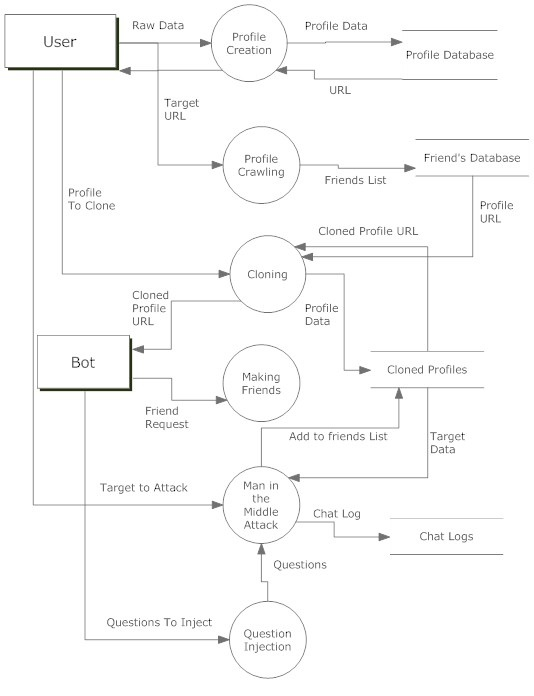
\includegraphics[scale=0.8]{project/diagrams/dfd2}
\caption{DFD - Level 2}
\label{fig:dfd2}
\end{figure}

\section{Activity Diagram}

\begin{figure}[H]
\centering
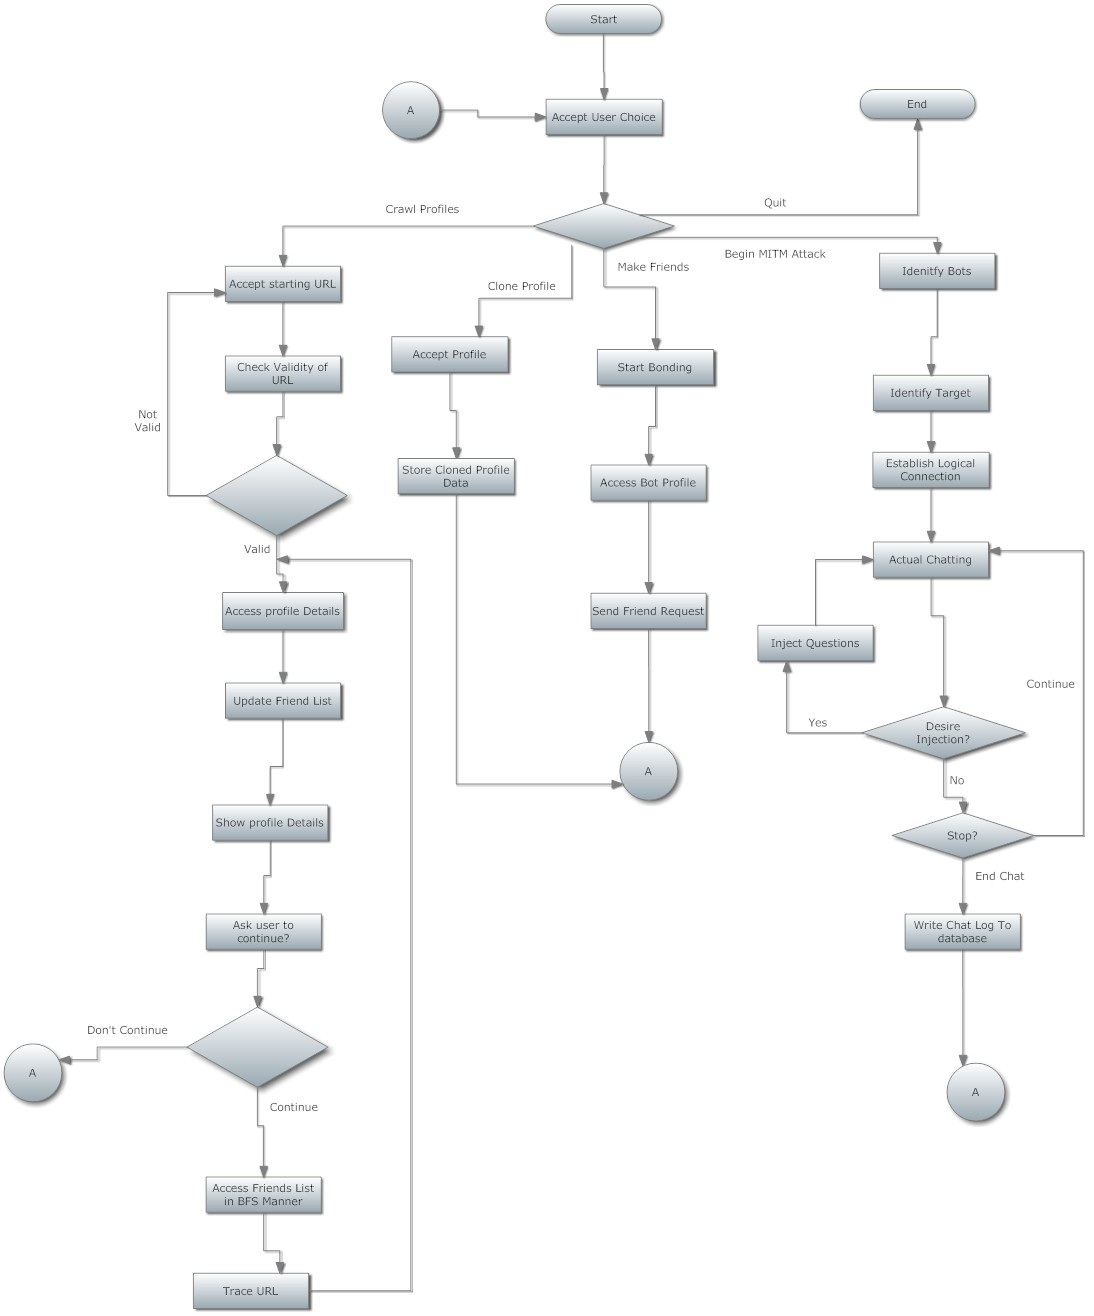
\includegraphics[scale=0.45]{project/diagrams/activity}
\caption{Activity Diagram}
\label{fig:activity}
\end{figure}


\section{Hardware and software requirements}
\subsection{Hardware}

%Add your items here
\begin{itemize}
\item{Standard Desktop Computer}
\item{2 GB Ram}
\item{80GB Hard Disk}
\item{Internet Connection}
\end{itemize}
\subsection{Software}

%This is how you add bullet points without a bullet
\begin{description}
\item[Operating System : ]  Any Linux based distro
\item[Language : ] Python 2.x
\item[Regular Expression : ] Python's re Library
\item[HTTP Requests : ] Python's urllib, urllib2 Library
\item[XMPP : ] Python's SleekXMPP Library
\end{description}

